\documentclass[1p]{elsarticle_modified}
%\bibliographystyle{elsarticle-num}

%\usepackage[colorlinks]{hyperref}
%\usepackage{abbrmath_seonhwa} %\Abb, \Ascr, \Acal ,\Abf, \Afrak
\usepackage{amsfonts}
\usepackage{amssymb}
\usepackage{amsmath}
\usepackage{amsthm}
\usepackage{scalefnt}
\usepackage{amsbsy}
\usepackage{kotex}
\usepackage{caption}
\usepackage{subfig}
\usepackage{color}
\usepackage{graphicx}
\usepackage{xcolor} %% white, black, red, green, blue, cyan, magenta, yellow
\usepackage{float}
\usepackage{setspace}
\usepackage{hyperref}

\usepackage{tikz}
\usetikzlibrary{arrows}

\usepackage{multirow}
\usepackage{array} % fixed length table
\usepackage{hhline}

%%%%%%%%%%%%%%%%%%%%%
\makeatletter
\renewcommand*\env@matrix[1][\arraystretch]{%
	\edef\arraystretch{#1}%
	\hskip -\arraycolsep
	\let\@ifnextchar\new@ifnextchar
	\array{*\c@MaxMatrixCols c}}
\makeatother %https://tex.stackexchange.com/questions/14071/how-can-i-increase-the-line-spacing-in-a-matrix
%%%%%%%%%%%%%%%

\usepackage[normalem]{ulem}

\newcommand{\msout}[1]{\ifmmode\text{\sout{\ensuremath{#1}}}\else\sout{#1}\fi}
%SOURCE: \msout is \stkout macro in https://tex.stackexchange.com/questions/20609/strikeout-in-math-mode

\newcommand{\cancel}[1]{
	\ifmmode
	{\color{red}\msout{#1}}
	\else
	{\color{red}\sout{#1}}
	\fi
}

\newcommand{\add}[1]{
	{\color{blue}\uwave{#1}}
}

\newcommand{\replace}[2]{
	\ifmmode
	{\color{red}\msout{#1}}{\color{blue}\uwave{#2}}
	\else
	{\color{red}\sout{#1}}{\color{blue}\uwave{#2}}
	\fi
}

\newcommand{\Sol}{\mathcal{S}} %segment
\newcommand{\D}{D} %diagram
\newcommand{\A}{\mathcal{A}} %arc


%%%%%%%%%%%%%%%%%%%%%%%%%%%%%5 test

\def\sl{\operatorname{\textup{SL}}(2,\Cbb)}
\def\psl{\operatorname{\textup{PSL}}(2,\Cbb)}
\def\quan{\mkern 1mu \triangleright \mkern 1mu}

\theoremstyle{definition}
\newtheorem{thm}{Theorem}[section]
\newtheorem{prop}[thm]{Proposition}
\newtheorem{lem}[thm]{Lemma}
\newtheorem{ques}[thm]{Question}
\newtheorem{cor}[thm]{Corollary}
\newtheorem{defn}[thm]{Definition}
\newtheorem{exam}[thm]{Example}
\newtheorem{rmk}[thm]{Remark}
\newtheorem{alg}[thm]{Algorithm}

\newcommand{\I}{\sqrt{-1}}
\begin{document}

%\begin{frontmatter}
%
%\title{Boundary parabolic representations of knots up to 8 crossings}
%
%%% Group authors per affiliation:
%\author{Yunhi Cho} 
%\address{Department of Mathematics, University of Seoul, Seoul, Korea}
%\ead{yhcho@uos.ac.kr}
%
%
%\author{Seonhwa Kim} %\fnref{s_kim}}
%\address{Center for Geometry and Physics, Institute for Basic Science, Pohang, 37673, Korea}
%\ead{ryeona17@ibs.re.kr}
%
%\author{Hyuk Kim}
%\address{Department of Mathematical Sciences, Seoul National University, Seoul 08826, Korea}
%\ead{hyukkim@snu.ac.kr}
%
%\author{Seokbeom Yoon}
%\address{Department of Mathematical Sciences, Seoul National University, Seoul, 08826,  Korea}
%\ead{sbyoon15@snu.ac.kr}
%
%\begin{abstract}
%We find all boundary parabolic representation of knots up to 8 crossings.
%
%\end{abstract}
%\begin{keyword}
%    \MSC[2010] 57M25 
%\end{keyword}
%
%\end{frontmatter}

%\linenumbers
%\tableofcontents
%
\newcommand\colored[1]{\textcolor{white}{\rule[-0.35ex]{0.8em}{1.4ex}}\kern-0.8em\color{red} #1}%
%\newcommand\colored[1]{\textcolor{white}{ #1}\kern-2.17ex	\textcolor{white}{ #1}\kern-1.81ex	\textcolor{white}{ #1}\kern-2.15ex\color{red}#1	}

{\Large $\underline{11a_{122}~(K11a_{122})}$}

\setlength{\tabcolsep}{10pt}
\renewcommand{\arraystretch}{1.6}
\vspace{1cm}\begin{tabular}{m{100pt}>{\centering\arraybackslash}m{274pt}}
\multirow{5}{120pt}{
	\centering
	\includegraphics[width=112pt]{../../../GIT/diagram.site/Diagrams/png/371_11a_122.png}\\
\ \ \ A knot diagram\footnotemark}&
\allowdisplaybreaks
\textbf{Linearized knot diagam} \\
\cline{2-2}
 &
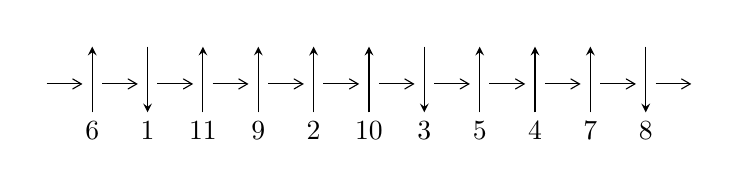
\begin{tikzpicture}[x=20pt, y=17pt]
	% nodes
	\node (C0) at (0, 0) {};
	\node (C1) at (1, 0) {};
	\node (C1U) at (1, +1) {};
	\node (C1D) at (1, -1) {6};

	\node (C2) at (2, 0) {};
	\node (C2U) at (2, +1) {};
	\node (C2D) at (2, -1) {1};

	\node (C3) at (3, 0) {};
	\node (C3U) at (3, +1) {};
	\node (C3D) at (3, -1) {11};

	\node (C4) at (4, 0) {};
	\node (C4U) at (4, +1) {};
	\node (C4D) at (4, -1) {9};

	\node (C5) at (5, 0) {};
	\node (C5U) at (5, +1) {};
	\node (C5D) at (5, -1) {2};

	\node (C6) at (6, 0) {};
	\node (C6U) at (6, +1) {};
	\node (C6D) at (6, -1) {10};

	\node (C7) at (7, 0) {};
	\node (C7U) at (7, +1) {};
	\node (C7D) at (7, -1) {3};

	\node (C8) at (8, 0) {};
	\node (C8U) at (8, +1) {};
	\node (C8D) at (8, -1) {5};

	\node (C9) at (9, 0) {};
	\node (C9U) at (9, +1) {};
	\node (C9D) at (9, -1) {4};

	\node (C10) at (10, 0) {};
	\node (C10U) at (10, +1) {};
	\node (C10D) at (10, -1) {7};

	\node (C11) at (11, 0) {};
	\node (C11U) at (11, +1) {};
	\node (C11D) at (11, -1) {8};
	\node (C12) at (12, 0) {};

	% arrows
	\draw[->,>={angle 60}]
	(C0) edge (C1) (C1) edge (C2) (C2) edge (C3) (C3) edge (C4) (C4) edge (C5) (C5) edge (C6) (C6) edge (C7) (C7) edge (C8) (C8) edge (C9) (C9) edge (C10) (C10) edge (C11) (C11) edge (C12) ;	\draw[->,>=stealth]
	(C1D) edge (C1U) (C2U) edge (C2D) (C3D) edge (C3U) (C4D) edge (C4U) (C5D) edge (C5U) (C6D) edge (C6U) (C7U) edge (C7D) (C8D) edge (C8U) (C9D) edge (C9U) (C10D) edge (C10U) (C11U) edge (C11D) ;
	\end{tikzpicture} \\
\hhline{~~} \\& 
\textbf{Solving Sequence} \\ \cline{2-2} 
 &
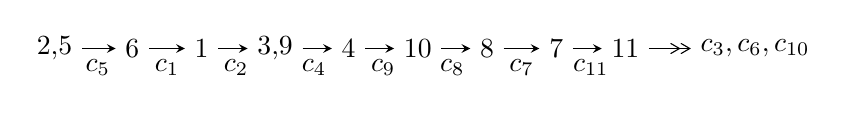
\begin{tikzpicture}[x=25pt, y=7pt]
	% node
	\node (A0) at (-1/8, 0) {2,5};
	\node (A1) at (1, 0) {6};
	\node (A2) at (2, 0) {1};
	\node (A3) at (49/16, 0) {3,9};
	\node (A4) at (33/8, 0) {4};
	\node (A5) at (41/8, 0) {10};
	\node (A6) at (49/8, 0) {8};
	\node (A7) at (57/8, 0) {7};
	\node (A8) at (65/8, 0) {11};
	\node (C1) at (1/2, -1) {$c_{5}$};
	\node (C2) at (3/2, -1) {$c_{1}$};
	\node (C3) at (5/2, -1) {$c_{2}$};
	\node (C4) at (29/8, -1) {$c_{4}$};
	\node (C5) at (37/8, -1) {$c_{9}$};
	\node (C6) at (45/8, -1) {$c_{8}$};
	\node (C7) at (53/8, -1) {$c_{7}$};
	\node (C8) at (61/8, -1) {$c_{11}$};
	\node (A9) at (10, 0) {$c_{3},c_{6},c_{10}$};

	% edge
	\draw[->,>=stealth]	
	(A0) edge (A1) (A1) edge (A2) (A2) edge (A3) (A3) edge (A4) (A4) edge (A5) (A5) edge (A6) (A6) edge (A7) (A7) edge (A8) ;
	\draw[->>,>={angle 60}]	
	(A8) edge (A9);
\end{tikzpicture} \\ 

\end{tabular} \\

\footnotetext{
The image of knot diagram is generated by the software ``\textbf{Draw programme}" developed by Andrew Bartholomew(\url{http://www.layer8.co.uk/maths/draw/index.htm\#Running-draw}), where we modified some parts for our purpose(\url{https://github.com/CATsTAILs/LinksPainter}).
}\phantom \\ \newline 
\centering \textbf{Ideals for irreducible components\footnotemark of $X_{\text{par}}$} 
 
\begin{align*}
I^u_{1}&=\langle 
1.11816\times10^{100} u^{76}+2.64440\times10^{100} u^{75}+\cdots+6.73504\times10^{100} b-1.22538\times10^{101},\\
\phantom{I^u_{1}}&\phantom{= \langle  }1.71883\times10^{101} u^{76}+1.13256\times10^{100} u^{75}+\cdots+6.73504\times10^{100} a+2.54056\times10^{102},\\
\phantom{I^u_{1}}&\phantom{= \langle  }u^{77}+17 u^{75}+\cdots+27 u-19\rangle \\
I^u_{2}&=\langle 
-2 u^{12}- u^{11}-6 u^{10}-2 u^9-12 u^8-3 u^7-16 u^6- u^5-17 u^4+u^3-9 u^2+b+u-2,\\
\phantom{I^u_{2}}&\phantom{= \langle  }- u^{13}-2 u^{12}-3 u^{11}-4 u^{10}-5 u^9-8 u^8-6 u^7-8 u^6-4 u^5-9 u^4-4 u^2+a+u-3,\\
\phantom{I^u_{2}}&\phantom{= \langle  }u^{14}+u^{13}+4 u^{12}+3 u^{11}+9 u^{10}+6 u^9+14 u^8+7 u^7+16 u^6+6 u^5+12 u^4+3 u^3+5 u^2+u+1\rangle \\
\\
\end{align*}
\raggedright * 2 irreducible components of $\dim_{\mathbb{C}}=0$, with total 91 representations.\\
\footnotetext{All coefficients of polynomials are rational numbers. But the coefficients are sometimes approximated in decimal forms when there is not enough margin.}
\newpage
\renewcommand{\arraystretch}{1}
\centering \section*{I. $I^u_{1}= \langle 1.12\times10^{100} u^{76}+2.64\times10^{100} u^{75}+\cdots+6.74\times10^{100} b-1.23\times10^{101},\;1.72\times10^{101} u^{76}+1.13\times10^{100} u^{75}+\cdots+6.74\times10^{100} a+2.54\times10^{102},\;u^{77}+17 u^{75}+\cdots+27 u-19 \rangle$}
\flushleft \textbf{(i) Arc colorings}\\
\begin{tabular}{m{7pt} m{180pt} m{7pt} m{180pt} }
\flushright $a_{2}=$&$\begin{pmatrix}0\\u\end{pmatrix}$ \\
\flushright $a_{5}=$&$\begin{pmatrix}1\\0\end{pmatrix}$ \\
\flushright $a_{6}=$&$\begin{pmatrix}1\\- u^2\end{pmatrix}$ \\
\flushright $a_{1}=$&$\begin{pmatrix}- u\\u^3+u\end{pmatrix}$ \\
\flushright $a_{3}=$&$\begin{pmatrix}- u^3\\u^5+u^3+u\end{pmatrix}$ \\
\flushright $a_{9}=$&$\begin{pmatrix}-2.55207 u^{76}-0.168159 u^{75}+\cdots+78.3494 u-37.7215\\-0.166022 u^{76}-0.392633 u^{75}+\cdots-4.69316 u+1.81941\end{pmatrix}$ \\
\flushright $a_{4}=$&$\begin{pmatrix}-0.359151 u^{76}-1.87506 u^{75}+\cdots-18.9968 u+37.8121\\0.319682 u^{76}+0.0483555 u^{75}+\cdots-4.22811 u+2.05086\end{pmatrix}$ \\
\flushright $a_{10}=$&$\begin{pmatrix}0.846949 u^{76}+0.811198 u^{75}+\cdots-10.8950 u-3.13453\\-0.402179 u^{76}-0.132584 u^{75}+\cdots+8.64112 u+0.469899\end{pmatrix}$ \\
\flushright $a_{8}=$&$\begin{pmatrix}-2.38605 u^{76}+0.224474 u^{75}+\cdots+83.0425 u-39.5409\\-0.166022 u^{76}-0.392633 u^{75}+\cdots-4.69316 u+1.81941\end{pmatrix}$ \\
\flushright $a_{7}=$&$\begin{pmatrix}-3.00143 u^{76}-0.717479 u^{75}+\cdots+89.2717 u-30.5770\\-0.417577 u^{76}-0.798995 u^{75}+\cdots-0.00895837 u+7.52176\end{pmatrix}$ \\
\flushright $a_{11}=$&$\begin{pmatrix}1.52003 u^{76}+1.34012 u^{75}+\cdots-26.0059 u+0.0397533\\-0.312532 u^{76}+0.595403 u^{75}+\cdots+23.5262 u-15.6637\end{pmatrix}$\\ \flushright $a_{11}=$&$\begin{pmatrix}1.52003 u^{76}+1.34012 u^{75}+\cdots-26.0059 u+0.0397533\\-0.312532 u^{76}+0.595403 u^{75}+\cdots+23.5262 u-15.6637\end{pmatrix}$\\&\end{tabular}
\flushleft \textbf{(ii) Obstruction class $= -1$}\\~\\
\flushleft \textbf{(iii) Cusp Shapes $= 2.91959 u^{76}+2.19877 u^{75}+\cdots-80.9270 u-2.56214$}\\~\\
\newpage\renewcommand{\arraystretch}{1}
\flushleft \textbf{(iv) u-Polynomials at the component}\newline \\
\begin{tabular}{m{50pt}|m{274pt}}
Crossings & \hspace{64pt}u-Polynomials at each crossing \\
\hline $$\begin{aligned}c_{1},c_{5}\end{aligned}$$&$\begin{aligned}
&u^{77}+17 u^{75}+\cdots+27 u-19
\end{aligned}$\\
\hline $$\begin{aligned}c_{2}\end{aligned}$$&$\begin{aligned}
&u^{77}+34 u^{76}+\cdots-5009 u-361
\end{aligned}$\\
\hline $$\begin{aligned}c_{3}\end{aligned}$$&$\begin{aligned}
&u^{77}+7 u^{76}+\cdots+18 u+1
\end{aligned}$\\
\hline $$\begin{aligned}c_{4},c_{8},c_{9}\end{aligned}$$&$\begin{aligned}
&u^{77}- u^{76}+\cdots+6 u-19
\end{aligned}$\\
\hline $$\begin{aligned}c_{6},c_{10}\end{aligned}$$&$\begin{aligned}
&u^{77}+u^{76}+\cdots+420 u-25
\end{aligned}$\\
\hline $$\begin{aligned}c_{7}\end{aligned}$$&$\begin{aligned}
&u^{77}- u^{76}+\cdots+138 u-323
\end{aligned}$\\
\hline $$\begin{aligned}c_{11}\end{aligned}$$&$\begin{aligned}
&u^{77}+5 u^{76}+\cdots-282 u-31
\end{aligned}$\\
\hline
\end{tabular}\\~\\
\newpage\renewcommand{\arraystretch}{1}
\flushleft \textbf{(v) Riley Polynomials at the component}\newline \\
\begin{tabular}{m{50pt}|m{274pt}}
Crossings & \hspace{64pt}Riley Polynomials at each crossing \\
\hline $$\begin{aligned}c_{1},c_{5}\end{aligned}$$&$\begin{aligned}
&y^{77}+34 y^{76}+\cdots-5009 y-361
\end{aligned}$\\
\hline $$\begin{aligned}c_{2}\end{aligned}$$&$\begin{aligned}
&y^{77}+26 y^{76}+\cdots+3771587 y-130321
\end{aligned}$\\
\hline $$\begin{aligned}c_{3}\end{aligned}$$&$\begin{aligned}
&y^{77}- y^{76}+\cdots-142 y-1
\end{aligned}$\\
\hline $$\begin{aligned}c_{4},c_{8},c_{9}\end{aligned}$$&$\begin{aligned}
&y^{77}+75 y^{76}+\cdots-3156 y-361
\end{aligned}$\\
\hline $$\begin{aligned}c_{6},c_{10}\end{aligned}$$&$\begin{aligned}
&y^{77}-49 y^{76}+\cdots+40050 y-625
\end{aligned}$\\
\hline $$\begin{aligned}c_{7}\end{aligned}$$&$\begin{aligned}
&y^{77}+21 y^{76}+\cdots-3986156 y-104329
\end{aligned}$\\
\hline $$\begin{aligned}c_{11}\end{aligned}$$&$\begin{aligned}
&y^{77}-3 y^{76}+\cdots+22112 y-961
\end{aligned}$\\
\hline
\end{tabular}\\~\\
\newpage\flushleft \textbf{(vi) Complex Volumes and Cusp Shapes}
$$\begin{array}{c|c|c}  
\text{Solutions to }I^u_{1}& \I (\text{vol} + \sqrt{-1}CS) & \text{Cusp shape}\\
 \hline 
\begin{aligned}
u &= -0.992506 + 0.102823 I \\
a &= \phantom{-}0.134683 + 1.153340 I \\
b &= \phantom{-}0.163116 + 1.299630 I\end{aligned}
 & \phantom{-}0.401797 + 0.602420 I & \phantom{-0.000000 } 0 \\ \hline\begin{aligned}
u &= -0.992506 - 0.102823 I \\
a &= \phantom{-}0.134683 - 1.153340 I \\
b &= \phantom{-}0.163116 - 1.299630 I\end{aligned}
 & \phantom{-}0.401797 - 0.602420 I & \phantom{-0.000000 } 0 \\ \hline\begin{aligned}
u &= -0.179722 + 0.986918 I \\
a &= \phantom{-}0.207589 + 0.902053 I \\
b &= \phantom{-}0.369165 + 0.668249 I\end{aligned}
 & -3.15064 + 0.31796 I & \phantom{-0.000000 } 0 \\ \hline\begin{aligned}
u &= -0.179722 - 0.986918 I \\
a &= \phantom{-}0.207589 - 0.902053 I \\
b &= \phantom{-}0.369165 - 0.668249 I\end{aligned}
 & -3.15064 - 0.31796 I & \phantom{-0.000000 } 0 \\ \hline\begin{aligned}
u &= -0.843840 + 0.510397 I \\
a &= -0.259951 - 0.265595 I \\
b &= \phantom{-}0.864185 + 0.337395 I\end{aligned}
 & \phantom{-}4.98057 + 6.15682 I & \phantom{-0.000000 } 0 \\ \hline\begin{aligned}
u &= -0.843840 - 0.510397 I \\
a &= -0.259951 + 0.265595 I \\
b &= \phantom{-}0.864185 - 0.337395 I\end{aligned}
 & \phantom{-}4.98057 - 6.15682 I & \phantom{-0.000000 } 0 \\ \hline\begin{aligned}
u &= -0.399420 + 0.898642 I \\
a &= -1.06991 - 2.30707 I \\
b &= -0.07605 - 1.75821 I\end{aligned}
 & -7.58964 - 1.63836 I & \phantom{-0.000000 } 0 \\ \hline\begin{aligned}
u &= -0.399420 - 0.898642 I \\
a &= -1.06991 + 2.30707 I \\
b &= -0.07605 + 1.75821 I\end{aligned}
 & -7.58964 + 1.63836 I & \phantom{-0.000000 } 0 \\ \hline\begin{aligned}
u &= \phantom{-}0.429893 + 0.940961 I \\
a &= \phantom{-}2.79308 - 2.27591 I \\
b &= -0.023408 - 1.309520 I\end{aligned}
 & -2.33844 - 1.16139 I & \phantom{-0.000000 } 0 \\ \hline\begin{aligned}
u &= \phantom{-}0.429893 - 0.940961 I \\
a &= \phantom{-}2.79308 + 2.27591 I \\
b &= -0.023408 + 1.309520 I\end{aligned}
 & -2.33844 + 1.16139 I & \phantom{-0.000000 } 0\\
 \hline 
 \end{array}$$\newpage$$\begin{array}{c|c|c}  
\text{Solutions to }I^u_{1}& \I (\text{vol} + \sqrt{-1}CS) & \text{Cusp shape}\\
 \hline 
\begin{aligned}
u &= \phantom{-}0.830555 + 0.488900 I \\
a &= \phantom{-}0.442225 + 0.331567 I \\
b &= -0.16770 + 1.41359 I\end{aligned}
 & -4.74914 - 4.01083 I & \phantom{-0.000000 } 0 \\ \hline\begin{aligned}
u &= \phantom{-}0.830555 - 0.488900 I \\
a &= \phantom{-}0.442225 - 0.331567 I \\
b &= -0.16770 - 1.41359 I\end{aligned}
 & -4.74914 + 4.01083 I & \phantom{-0.000000 } 0 \\ \hline\begin{aligned}
u &= -0.630106 + 0.842299 I \\
a &= \phantom{-}0.432588 - 0.361290 I \\
b &= -0.622284 - 0.227967 I\end{aligned}
 & \phantom{-}3.97239 - 0.95647 I & \phantom{-0.000000 } 0 \\ \hline\begin{aligned}
u &= -0.630106 - 0.842299 I \\
a &= \phantom{-}0.432588 + 0.361290 I \\
b &= -0.622284 + 0.227967 I\end{aligned}
 & \phantom{-}3.97239 + 0.95647 I & \phantom{-0.000000 } 0 \\ \hline\begin{aligned}
u &= \phantom{-}0.303925 + 0.883906 I \\
a &= \phantom{-}0.690866 - 1.050320 I \\
b &= -0.870665 - 0.383585 I\end{aligned}
 & \phantom{-}0.163595 - 0.350353 I & \phantom{-0.000000 } 0 \\ \hline\begin{aligned}
u &= \phantom{-}0.303925 - 0.883906 I \\
a &= \phantom{-}0.690866 + 1.050320 I \\
b &= -0.870665 + 0.383585 I\end{aligned}
 & \phantom{-}0.163595 + 0.350353 I & \phantom{-0.000000 } 0 \\ \hline\begin{aligned}
u &= \phantom{-}0.934821 + 0.515588 I \\
a &= -0.0267477 - 0.1090470 I \\
b &= \phantom{-}0.527513 - 0.109138 I\end{aligned}
 & \phantom{-}4.74218 + 1.96042 I & \phantom{-0.000000 } 0 \\ \hline\begin{aligned}
u &= \phantom{-}0.934821 - 0.515588 I \\
a &= -0.0267477 + 0.1090470 I \\
b &= \phantom{-}0.527513 + 0.109138 I\end{aligned}
 & \phantom{-}4.74218 - 1.96042 I & \phantom{-0.000000 } 0 \\ \hline\begin{aligned}
u &= -0.659420 + 0.849922 I \\
a &= -0.48497 - 1.38896 I \\
b &= \phantom{-}0.432084 - 0.317596 I\end{aligned}
 & \phantom{-}3.96385 - 4.06799 I & \phantom{-0.000000 } 0 \\ \hline\begin{aligned}
u &= -0.659420 - 0.849922 I \\
a &= -0.48497 + 1.38896 I \\
b &= \phantom{-}0.432084 + 0.317596 I\end{aligned}
 & \phantom{-}3.96385 + 4.06799 I & \phantom{-0.000000 } 0\\
 \hline 
 \end{array}$$\newpage$$\begin{array}{c|c|c}  
\text{Solutions to }I^u_{1}& \I (\text{vol} + \sqrt{-1}CS) & \text{Cusp shape}\\
 \hline 
\begin{aligned}
u &= \phantom{-}0.989911 + 0.422296 I \\
a &= -0.202342 - 0.690980 I \\
b &= \phantom{-}0.32715 - 1.45728 I\end{aligned}
 & -0.76965 - 10.43430 I & \phantom{-0.000000 } 0 \\ \hline\begin{aligned}
u &= \phantom{-}0.989911 - 0.422296 I \\
a &= -0.202342 + 0.690980 I \\
b &= \phantom{-}0.32715 + 1.45728 I\end{aligned}
 & -0.76965 + 10.43430 I & \phantom{-0.000000 } 0 \\ \hline\begin{aligned}
u &= \phantom{-}0.509665 + 0.956039 I \\
a &= -1.85319 + 2.97020 I \\
b &= \phantom{-}0.17312 + 1.44644 I\end{aligned}
 & -1.80643 + 6.36048 I & \phantom{-0.000000 } 0 \\ \hline\begin{aligned}
u &= \phantom{-}0.509665 - 0.956039 I \\
a &= -1.85319 - 2.97020 I \\
b &= \phantom{-}0.17312 - 1.44644 I\end{aligned}
 & -1.80643 - 6.36048 I & \phantom{-0.000000 } 0 \\ \hline\begin{aligned}
u &= \phantom{-}0.435143 + 1.013860 I \\
a &= \phantom{-}0.085209 + 0.808618 I \\
b &= \phantom{-}0.861923 - 0.018150 I\end{aligned}
 & -0.79562 + 3.15505 I & \phantom{-0.000000 } 0 \\ \hline\begin{aligned}
u &= \phantom{-}0.435143 - 1.013860 I \\
a &= \phantom{-}0.085209 - 0.808618 I \\
b &= \phantom{-}0.861923 + 0.018150 I\end{aligned}
 & -0.79562 - 3.15505 I & \phantom{-0.000000 } 0 \\ \hline\begin{aligned}
u &= \phantom{-}0.629756 + 0.623375 I \\
a &= -1.03801 + 1.27838 I \\
b &= \phantom{-}0.698651 + 0.940608 I\end{aligned}
 & \phantom{-}3.26953 - 0.81616 I & \phantom{-}8.32679 + 0.51400 I \\ \hline\begin{aligned}
u &= \phantom{-}0.629756 - 0.623375 I \\
a &= -1.03801 - 1.27838 I \\
b &= \phantom{-}0.698651 - 0.940608 I\end{aligned}
 & \phantom{-}3.26953 + 0.81616 I & \phantom{-}8.32679 - 0.51400 I \\ \hline\begin{aligned}
u &= \phantom{-}0.478152 + 1.028480 I \\
a &= \phantom{-}0.048348 + 0.408631 I \\
b &= \phantom{-}0.620681 - 0.234635 I\end{aligned}
 & -0.64979 + 3.08848 I & \phantom{-0.000000 } 0 \\ \hline\begin{aligned}
u &= \phantom{-}0.478152 - 1.028480 I \\
a &= \phantom{-}0.048348 - 0.408631 I \\
b &= \phantom{-}0.620681 + 0.234635 I\end{aligned}
 & -0.64979 - 3.08848 I & \phantom{-0.000000 } 0\\
 \hline 
 \end{array}$$\newpage$$\begin{array}{c|c|c}  
\text{Solutions to }I^u_{1}& \I (\text{vol} + \sqrt{-1}CS) & \text{Cusp shape}\\
 \hline 
\begin{aligned}
u &= \phantom{-}0.474736 + 0.723995 I \\
a &= \phantom{-}0.76434 + 1.28908 I \\
b &= -0.256829 + 1.358870 I\end{aligned}
 & -1.02736 - 2.28684 I & \phantom{-}7.55737 - 1.92002 I \\ \hline\begin{aligned}
u &= \phantom{-}0.474736 - 0.723995 I \\
a &= \phantom{-}0.76434 - 1.28908 I \\
b &= -0.256829 - 1.358870 I\end{aligned}
 & -1.02736 + 2.28684 I & \phantom{-}7.55737 + 1.92002 I \\ \hline\begin{aligned}
u &= \phantom{-}0.095485 + 1.136580 I \\
a &= -0.502266 - 0.275607 I \\
b &= -0.410820 - 0.500865 I\end{aligned}
 & -1.23115 + 4.61547 I & \phantom{-0.000000 } 0 \\ \hline\begin{aligned}
u &= \phantom{-}0.095485 - 1.136580 I \\
a &= -0.502266 + 0.275607 I \\
b &= -0.410820 + 0.500865 I\end{aligned}
 & -1.23115 - 4.61547 I & \phantom{-0.000000 } 0 \\ \hline\begin{aligned}
u &= -0.545977 + 1.014860 I \\
a &= \phantom{-}1.60168 + 1.42484 I \\
b &= -0.25443 + 1.49778 I\end{aligned}
 & -6.23573 - 3.59828 I & \phantom{-0.000000 } 0 \\ \hline\begin{aligned}
u &= -0.545977 - 1.014860 I \\
a &= \phantom{-}1.60168 - 1.42484 I \\
b &= -0.25443 - 1.49778 I\end{aligned}
 & -6.23573 + 3.59828 I & \phantom{-0.000000 } 0 \\ \hline\begin{aligned}
u &= \phantom{-}0.582278 + 0.996325 I \\
a &= -0.563794 + 0.223191 I \\
b &= -0.890522 + 0.862779 I\end{aligned}
 & \phantom{-}2.13289 + 5.59350 I & \phantom{-0.000000 } 0 \\ \hline\begin{aligned}
u &= \phantom{-}0.582278 - 0.996325 I \\
a &= -0.563794 - 0.223191 I \\
b &= -0.890522 - 0.862779 I\end{aligned}
 & \phantom{-}2.13289 - 5.59350 I & \phantom{-0.000000 } 0 \\ \hline\begin{aligned}
u &= -0.670483 + 0.483183 I \\
a &= \phantom{-}0.434095 + 0.052172 I \\
b &= \phantom{-}0.091326 + 1.398830 I\end{aligned}
 & -4.69637 - 1.06019 I & \phantom{-}1.77167 + 3.37054 I \\ \hline\begin{aligned}
u &= -0.670483 - 0.483183 I \\
a &= \phantom{-}0.434095 - 0.052172 I \\
b &= \phantom{-}0.091326 - 1.398830 I\end{aligned}
 & -4.69637 + 1.06019 I & \phantom{-}1.77167 - 3.37054 I\\
 \hline 
 \end{array}$$\newpage$$\begin{array}{c|c|c}  
\text{Solutions to }I^u_{1}& \I (\text{vol} + \sqrt{-1}CS) & \text{Cusp shape}\\
 \hline 
\begin{aligned}
u &= \phantom{-}0.286414 + 0.770897 I \\
a &= -0.529133 + 0.340802 I \\
b &= -0.131537 - 1.082870 I\end{aligned}
 & -1.66948 + 4.41582 I & \phantom{-}1.89095 - 7.51021 I \\ \hline\begin{aligned}
u &= \phantom{-}0.286414 - 0.770897 I \\
a &= -0.529133 - 0.340802 I \\
b &= -0.131537 + 1.082870 I\end{aligned}
 & -1.66948 - 4.41582 I & \phantom{-}1.89095 + 7.51021 I \\ \hline\begin{aligned}
u &= \phantom{-}0.076124 + 1.176170 I \\
a &= -0.13232 - 2.63415 I \\
b &= \phantom{-}0.08777 - 1.53585 I\end{aligned}
 & -10.45230 - 1.94264 I & \phantom{-0.000000 } 0 \\ \hline\begin{aligned}
u &= \phantom{-}0.076124 - 1.176170 I \\
a &= -0.13232 + 2.63415 I \\
b &= \phantom{-}0.08777 + 1.53585 I\end{aligned}
 & -10.45230 + 1.94264 I & \phantom{-0.000000 } 0 \\ \hline\begin{aligned}
u &= -0.574941 + 1.029820 I \\
a &= -0.865274 - 0.836985 I \\
b &= \phantom{-}0.601944 - 0.367094 I\end{aligned}
 & -0.73372 - 6.46640 I & \phantom{-0.000000 } 0 \\ \hline\begin{aligned}
u &= -0.574941 - 1.029820 I \\
a &= -0.865274 + 0.836985 I \\
b &= \phantom{-}0.601944 + 0.367094 I\end{aligned}
 & -0.73372 + 6.46640 I & \phantom{-0.000000 } 0 \\ \hline\begin{aligned}
u &= -0.331830 + 1.139990 I \\
a &= \phantom{-}0.81647 + 2.00240 I \\
b &= \phantom{-}0.22724 + 1.48431 I\end{aligned}
 & -6.59087 + 0.43258 I & \phantom{-0.000000 } 0 \\ \hline\begin{aligned}
u &= -0.331830 - 1.139990 I \\
a &= \phantom{-}0.81647 - 2.00240 I \\
b &= \phantom{-}0.22724 - 1.48431 I\end{aligned}
 & -6.59087 - 0.43258 I & \phantom{-0.000000 } 0 \\ \hline\begin{aligned}
u &= \phantom{-}0.799696 + 0.881266 I \\
a &= \phantom{-}0.800094 + 0.035250 I \\
b &= -0.025687 - 1.228280 I\end{aligned}
 & \phantom{-}1.67283 + 2.99269 I & \phantom{-0.000000 } 0 \\ \hline\begin{aligned}
u &= \phantom{-}0.799696 - 0.881266 I \\
a &= \phantom{-}0.800094 - 0.035250 I \\
b &= -0.025687 + 1.228280 I\end{aligned}
 & \phantom{-}1.67283 - 2.99269 I & \phantom{-0.000000 } 0\\
 \hline 
 \end{array}$$\newpage$$\begin{array}{c|c|c}  
\text{Solutions to }I^u_{1}& \I (\text{vol} + \sqrt{-1}CS) & \text{Cusp shape}\\
 \hline 
\begin{aligned}
u &= -0.503300 + 1.113020 I \\
a &= -1.46906 - 1.97320 I \\
b &= \phantom{-}0.43026 - 1.43315 I\end{aligned}
 & -5.46055 - 8.15782 I & \phantom{-0.000000 } 0 \\ \hline\begin{aligned}
u &= -0.503300 - 1.113020 I \\
a &= -1.46906 + 1.97320 I \\
b &= \phantom{-}0.43026 + 1.43315 I\end{aligned}
 & -5.46055 + 8.15782 I & \phantom{-0.000000 } 0 \\ \hline\begin{aligned}
u &= -0.588221 + 0.492828 I \\
a &= \phantom{-}1.010850 + 0.219431 I \\
b &= -0.413424 - 0.322512 I\end{aligned}
 & \phantom{-}0.78679 + 1.78171 I & \phantom{-}6.93161 - 4.77332 I \\ \hline\begin{aligned}
u &= -0.588221 - 0.492828 I \\
a &= \phantom{-}1.010850 - 0.219431 I \\
b &= -0.413424 + 0.322512 I\end{aligned}
 & \phantom{-}0.78679 - 1.78171 I & \phantom{-}6.93161 + 4.77332 I \\ \hline\begin{aligned}
u &= -0.654044 + 1.088480 I \\
a &= \phantom{-}0.275617 + 1.042120 I \\
b &= -0.951503 + 0.450492 I\end{aligned}
 & \phantom{-}3.22901 - 11.73080 I & \phantom{-0.000000 } 0 \\ \hline\begin{aligned}
u &= -0.654044 - 1.088480 I \\
a &= \phantom{-}0.275617 - 1.042120 I \\
b &= -0.951503 - 0.450492 I\end{aligned}
 & \phantom{-}3.22901 + 11.73080 I & \phantom{-0.000000 } 0 \\ \hline\begin{aligned}
u &= \phantom{-}0.651187 + 1.101690 I \\
a &= -1.82390 + 1.46274 I \\
b &= \phantom{-}0.23240 + 1.44840 I\end{aligned}
 & -6.58950 + 9.55660 I & \phantom{-0.000000 } 0 \\ \hline\begin{aligned}
u &= \phantom{-}0.651187 - 1.101690 I \\
a &= -1.82390 - 1.46274 I \\
b &= \phantom{-}0.23240 - 1.44840 I\end{aligned}
 & -6.58950 - 9.55660 I & \phantom{-0.000000 } 0 \\ \hline\begin{aligned}
u &= \phantom{-}0.734204 + 1.069320 I \\
a &= \phantom{-}0.264381 - 0.642265 I \\
b &= -0.461381 - 0.424979 I\end{aligned}
 & \phantom{-}3.10184 + 4.12640 I & \phantom{-0.000000 } 0 \\ \hline\begin{aligned}
u &= \phantom{-}0.734204 - 1.069320 I \\
a &= \phantom{-}0.264381 + 0.642265 I \\
b &= -0.461381 + 0.424979 I\end{aligned}
 & \phantom{-}3.10184 - 4.12640 I & \phantom{-0.000000 } 0\\
 \hline 
 \end{array}$$\newpage$$\begin{array}{c|c|c}  
\text{Solutions to }I^u_{1}& \I (\text{vol} + \sqrt{-1}CS) & \text{Cusp shape}\\
 \hline 
\begin{aligned}
u &= \phantom{-}0.463474 + 0.499512 I \\
a &= \phantom{-}1.005840 - 0.131908 I \\
b &= -0.391996 - 0.381119 I\end{aligned}
 & \phantom{-}0.906262 + 0.882340 I & \phantom{-}7.93772 - 5.58390 I \\ \hline\begin{aligned}
u &= \phantom{-}0.463474 - 0.499512 I \\
a &= \phantom{-}1.005840 + 0.131908 I \\
b &= -0.391996 + 0.381119 I\end{aligned}
 & \phantom{-}0.906262 - 0.882340 I & \phantom{-}7.93772 + 5.58390 I \\ \hline\begin{aligned}
u &= -0.655837 + 0.159805 I \\
a &= \phantom{-}0.540689 - 0.181974 I \\
b &= -0.322778 - 1.352790 I\end{aligned}
 & -2.86462 + 3.78073 I & \phantom{-}3.56597 - 3.81882 I \\ \hline\begin{aligned}
u &= -0.655837 - 0.159805 I \\
a &= \phantom{-}0.540689 + 0.181974 I \\
b &= -0.322778 + 1.352790 I\end{aligned}
 & -2.86462 - 3.78073 I & \phantom{-}3.56597 + 3.81882 I \\ \hline\begin{aligned}
u &= \phantom{-}0.674571 + 1.175150 I \\
a &= \phantom{-}1.41651 - 1.82923 I \\
b &= -0.35663 - 1.51897 I\end{aligned}
 & -3.0941 + 16.4594 I & \phantom{-0.000000 } 0 \\ \hline\begin{aligned}
u &= \phantom{-}0.674571 - 1.175150 I \\
a &= \phantom{-}1.41651 + 1.82923 I \\
b &= -0.35663 + 1.51897 I\end{aligned}
 & -3.0941 - 16.4594 I & \phantom{-0.000000 } 0 \\ \hline\begin{aligned}
u &= -0.534948 + 1.254540 I \\
a &= -1.24467 - 1.97836 I \\
b &= \phantom{-}0.040134 - 1.286720 I\end{aligned}
 & -3.56674 - 4.58685 I & \phantom{-0.000000 } 0 \\ \hline\begin{aligned}
u &= -0.534948 - 1.254540 I \\
a &= -1.24467 + 1.97836 I \\
b &= \phantom{-}0.040134 + 1.286720 I\end{aligned}
 & -3.56674 + 4.58685 I & \phantom{-0.000000 } 0 \\ \hline\begin{aligned}
u &= \phantom{-}0.040521 + 1.392890 I \\
a &= -0.13926 + 2.26692 I \\
b &= -0.18547 + 1.46609 I\end{aligned}
 & -7.50502 - 7.02191 I & \phantom{-0.000000 } 0 \\ \hline\begin{aligned}
u &= \phantom{-}0.040521 - 1.392890 I \\
a &= -0.13926 - 2.26692 I \\
b &= -0.18547 - 1.46609 I\end{aligned}
 & -7.50502 + 7.02191 I & \phantom{-0.000000 } 0\\
 \hline 
 \end{array}$$\newpage$$\begin{array}{c|c|c}  
\text{Solutions to }I^u_{1}& \I (\text{vol} + \sqrt{-1}CS) & \text{Cusp shape}\\
 \hline 
\begin{aligned}
u &= -1.12911 + 0.85261 I \\
a &= -0.402883 - 0.940773 I \\
b &= \phantom{-}0.075532 - 1.274920 I\end{aligned}
 & \phantom{-}1.39277 - 3.88492 I & \phantom{-0.000000 } 0 \\ \hline\begin{aligned}
u &= -1.12911 - 0.85261 I \\
a &= -0.402883 + 0.940773 I \\
b &= \phantom{-}0.075532 + 1.274920 I\end{aligned}
 & \phantom{-}1.39277 + 3.88492 I & \phantom{-0.000000 } 0 \\ \hline\begin{aligned}
u &= -0.071474 + 0.574838 I \\
a &= \phantom{-}2.49648 + 0.24444 I \\
b &= \phantom{-}0.025774 - 0.381419 I\end{aligned}
 & \phantom{-}0.98061 + 1.39590 I & \phantom{-}4.58324 - 5.64184 I \\ \hline\begin{aligned}
u &= -0.071474 - 0.574838 I \\
a &= \phantom{-}2.49648 - 0.24444 I \\
b &= \phantom{-}0.025774 + 0.381419 I\end{aligned}
 & \phantom{-}0.98061 - 1.39590 I & \phantom{-}4.58324 + 5.64184 I \\ \hline\begin{aligned}
u &= -0.65986 + 1.27360 I \\
a &= \phantom{-}0.92752 + 2.00650 I \\
b &= -0.18093 + 1.46647 I\end{aligned}
 & -3.02971 - 6.56618 I & \phantom{-0.000000 } 0 \\ \hline\begin{aligned}
u &= -0.65986 - 1.27360 I \\
a &= \phantom{-}0.92752 - 2.00650 I \\
b &= -0.18093 - 1.46647 I\end{aligned}
 & -3.02971 + 6.56618 I & \phantom{-0.000000 } 0 \\ \hline\begin{aligned}
u &= \phantom{-}0.409048\phantom{ +0.000000I} \\
a &= \phantom{-}1.15285\phantom{ +0.000000I} \\
b &= -0.711871\phantom{ +0.000000I}\end{aligned}
 & \phantom{-}1.45831\phantom{ +0.000000I} & \phantom{-}6.75650\phantom{ +0.000000I}\\
 \hline 
 \end{array}$$\newpage\newpage\renewcommand{\arraystretch}{1}
\centering \section*{II. $I^u_{2}= \langle -2 u^{12}- u^{11}+\cdots+b-2,\;- u^{13}-2 u^{12}+\cdots+a-3,\;u^{14}+u^{13}+\cdots+u+1 \rangle$}
\flushleft \textbf{(i) Arc colorings}\\
\begin{tabular}{m{7pt} m{180pt} m{7pt} m{180pt} }
\flushright $a_{2}=$&$\begin{pmatrix}0\\u\end{pmatrix}$ \\
\flushright $a_{5}=$&$\begin{pmatrix}1\\0\end{pmatrix}$ \\
\flushright $a_{6}=$&$\begin{pmatrix}1\\- u^2\end{pmatrix}$ \\
\flushright $a_{1}=$&$\begin{pmatrix}- u\\u^3+u\end{pmatrix}$ \\
\flushright $a_{3}=$&$\begin{pmatrix}- u^3\\u^5+u^3+u\end{pmatrix}$ \\
\flushright $a_{9}=$&$\begin{pmatrix}u^{13}+2 u^{12}+\cdots- u+3\\2 u^{12}+u^{11}+\cdots- u+2\end{pmatrix}$ \\
\flushright $a_{4}=$&$\begin{pmatrix}u^{13}+3 u^{12}+\cdots- u+3\\- u^{12}- u^{11}-3 u^{10}-2 u^9-6 u^8-4 u^7-8 u^6-3 u^5-8 u^4-3 u^3-4 u^2-2\end{pmatrix}$ \\
\flushright $a_{10}=$&$\begin{pmatrix}-3 u^{12}-3 u^{11}+\cdots-4 u-4\\u^{13}- u^{12}+\cdots+u-2\end{pmatrix}$ \\
\flushright $a_{8}=$&$\begin{pmatrix}u^{13}+2 u^{11}-2 u^{10}+3 u^9-4 u^8+3 u^7-8 u^6+3 u^5-8 u^4+u^3-5 u^2+1\\2 u^{12}+u^{11}+\cdots- u+2\end{pmatrix}$ \\
\flushright $a_{7}=$&$\begin{pmatrix}u^{13}+u^{12}+\cdots-4 u^2+1\\2 u^{12}+u^{11}+\cdots- u+2\end{pmatrix}$ \\
\flushright $a_{11}=$&$\begin{pmatrix}u^{13}-2 u^{12}+\cdots+5 u-2\\u^{13}+3 u^{11}+6 u^9+8 u^7- u^6+9 u^5-2 u^4+6 u^3+u+1\end{pmatrix}$\\ \flushright $a_{11}=$&$\begin{pmatrix}u^{13}-2 u^{12}+\cdots+5 u-2\\u^{13}+3 u^{11}+6 u^9+8 u^7- u^6+9 u^5-2 u^4+6 u^3+u+1\end{pmatrix}$\\&\end{tabular}
\flushleft \textbf{(ii) Obstruction class $= 1$}\\~\\
\flushleft \textbf{(iii) Cusp Shapes $= - u^{13}-3 u^{12}-7 u^{11}-7 u^{10}-15 u^9-13 u^8-27 u^7-15 u^6-29 u^5-11 u^4-29 u^3-2 u^2-11 u+4$}\\~\\
\newpage\renewcommand{\arraystretch}{1}
\flushleft \textbf{(iv) u-Polynomials at the component}\newline \\
\begin{tabular}{m{50pt}|m{274pt}}
Crossings & \hspace{64pt}u-Polynomials at each crossing \\
\hline $$\begin{aligned}c_{1}\end{aligned}$$&$\begin{aligned}
&u^{14}- u^{13}+\cdots- u+1
\end{aligned}$\\
\hline $$\begin{aligned}c_{2}\end{aligned}$$&$\begin{aligned}
&u^{14}+7 u^{13}+\cdots+9 u+1
\end{aligned}$\\
\hline $$\begin{aligned}c_{3}\end{aligned}$$&$\begin{aligned}
&u^{14}+2 u^{11}-2 u^{10}+2 u^8-6 u^7+4 u^6+2 u^5-4 u^4+2 u^3+u^2-2 u+1
\end{aligned}$\\
\hline $$\begin{aligned}c_{4}\end{aligned}$$&$\begin{aligned}
&u^{14}+8 u^{12}+\cdots+4 u^2+1
\end{aligned}$\\
\hline $$\begin{aligned}c_{5}\end{aligned}$$&$\begin{aligned}
&u^{14}+u^{13}+\cdots+u+1
\end{aligned}$\\
\hline $$\begin{aligned}c_{6}\end{aligned}$$&$\begin{aligned}
&u^{14}-2 u^{13}+\cdots-2 u+1
\end{aligned}$\\
\hline $$\begin{aligned}c_{7}\end{aligned}$$&$\begin{aligned}
&u^{14}+3 u^{12}+\cdots+4 u^2+1
\end{aligned}$\\
\hline $$\begin{aligned}c_{8},c_{9}\end{aligned}$$&$\begin{aligned}
&u^{14}+8 u^{12}+\cdots+4 u^2+1
\end{aligned}$\\
\hline $$\begin{aligned}c_{10}\end{aligned}$$&$\begin{aligned}
&u^{14}+2 u^{13}+\cdots+2 u+1
\end{aligned}$\\
\hline $$\begin{aligned}c_{11}\end{aligned}$$&$\begin{aligned}
&u^{14}+u^{12}-3 u^{11}-2 u^{10}-2 u^9+u^8+3 u^7+5 u^6+u^5+u^4-2 u^3+1
\end{aligned}$\\
\hline
\end{tabular}\\~\\
\newpage\renewcommand{\arraystretch}{1}
\flushleft \textbf{(v) Riley Polynomials at the component}\newline \\
\begin{tabular}{m{50pt}|m{274pt}}
Crossings & \hspace{64pt}Riley Polynomials at each crossing \\
\hline $$\begin{aligned}c_{1},c_{5}\end{aligned}$$&$\begin{aligned}
&y^{14}+7 y^{13}+\cdots+9 y+1
\end{aligned}$\\
\hline $$\begin{aligned}c_{2}\end{aligned}$$&$\begin{aligned}
&y^{14}+7 y^{13}+\cdots+5 y+1
\end{aligned}$\\
\hline $$\begin{aligned}c_{3}\end{aligned}$$&$\begin{aligned}
&y^{14}-4 y^{12}+\cdots-2 y+1
\end{aligned}$\\
\hline $$\begin{aligned}c_{4},c_{8},c_{9}\end{aligned}$$&$\begin{aligned}
&y^{14}+16 y^{13}+\cdots+8 y+1
\end{aligned}$\\
\hline $$\begin{aligned}c_{6},c_{10}\end{aligned}$$&$\begin{aligned}
&y^{14}-12 y^{13}+\cdots-14 y+1
\end{aligned}$\\
\hline $$\begin{aligned}c_{7}\end{aligned}$$&$\begin{aligned}
&y^{14}+6 y^{13}+\cdots+8 y+1
\end{aligned}$\\
\hline $$\begin{aligned}c_{11}\end{aligned}$$&$\begin{aligned}
&y^{14}+2 y^{13}+\cdots+2 y^2+1
\end{aligned}$\\
\hline
\end{tabular}\\~\\
\newpage\flushleft \textbf{(vi) Complex Volumes and Cusp Shapes}
$$\begin{array}{c|c|c}  
\text{Solutions to }I^u_{2}& \I (\text{vol} + \sqrt{-1}CS) & \text{Cusp shape}\\
 \hline 
\begin{aligned}
u &= -0.263802 + 0.940835 I \\
a &= \phantom{-}1.19274 + 2.28120 I \\
b &= \phantom{-}0.04502 + 1.68553 I\end{aligned}
 & -8.10462 - 1.08865 I & -3.05079 - 1.27103 I \\ \hline\begin{aligned}
u &= -0.263802 - 0.940835 I \\
a &= \phantom{-}1.19274 - 2.28120 I \\
b &= \phantom{-}0.04502 - 1.68553 I\end{aligned}
 & -8.10462 + 1.08865 I & -3.05079 + 1.27103 I \\ \hline\begin{aligned}
u &= \phantom{-}0.410511 + 1.042370 I \\
a &= \phantom{-}0.131453 + 0.695630 I \\
b &= \phantom{-}0.588176 - 0.305776 I\end{aligned}
 & -0.04552 + 3.64299 I & \phantom{-}9.10899 - 6.17803 I \\ \hline\begin{aligned}
u &= \phantom{-}0.410511 - 1.042370 I \\
a &= \phantom{-}0.131453 - 0.695630 I \\
b &= \phantom{-}0.588176 + 0.305776 I\end{aligned}
 & -0.04552 - 3.64299 I & \phantom{-}9.10899 + 6.17803 I \\ \hline\begin{aligned}
u &= \phantom{-}0.760930 + 0.850713 I \\
a &= -0.428317 + 0.669340 I \\
b &= -0.100644 + 0.531390 I\end{aligned}
 & \phantom{-}3.68757 + 2.89359 I & \phantom{-}10.43723 - 2.39081 I \\ \hline\begin{aligned}
u &= \phantom{-}0.760930 - 0.850713 I \\
a &= -0.428317 - 0.669340 I \\
b &= -0.100644 - 0.531390 I\end{aligned}
 & \phantom{-}3.68757 - 2.89359 I & \phantom{-}10.43723 + 2.39081 I \\ \hline\begin{aligned}
u &= \phantom{-}0.312796 + 0.732458 I \\
a &= \phantom{-}1.95777 - 1.12081 I \\
b &= -0.492123 - 0.518251 I\end{aligned}
 & \phantom{-}1.193900 - 0.561188 I & \phantom{-}7.81743 - 1.40333 I \\ \hline\begin{aligned}
u &= \phantom{-}0.312796 - 0.732458 I \\
a &= \phantom{-}1.95777 + 1.12081 I \\
b &= -0.492123 + 0.518251 I\end{aligned}
 & \phantom{-}1.193900 + 0.561188 I & \phantom{-}7.81743 + 1.40333 I \\ \hline\begin{aligned}
u &= -0.942798 + 0.813476 I \\
a &= \phantom{-}0.324386 + 0.502415 I \\
b &= -0.045526 + 1.274860 I\end{aligned}
 & \phantom{-}0.85500 - 3.43645 I & \phantom{-}1.10715 + 2.59332 I \\ \hline\begin{aligned}
u &= -0.942798 - 0.813476 I \\
a &= \phantom{-}0.324386 - 0.502415 I \\
b &= -0.045526 - 1.274860 I\end{aligned}
 & \phantom{-}0.85500 + 3.43645 I & \phantom{-}1.10715 - 2.59332 I\\
 \hline 
 \end{array}$$\newpage$$\begin{array}{c|c|c}  
\text{Solutions to }I^u_{2}& \I (\text{vol} + \sqrt{-1}CS) & \text{Cusp shape}\\
 \hline 
\begin{aligned}
u &= -0.495691 + 1.193760 I \\
a &= -1.17726 - 2.37223 I \\
b &= \phantom{-}0.19941 - 1.40134 I\end{aligned}
 & -4.20321 - 6.46120 I & \phantom{-}0.62933 + 6.25768 I \\ \hline\begin{aligned}
u &= -0.495691 - 1.193760 I \\
a &= -1.17726 + 2.37223 I \\
b &= \phantom{-}0.19941 + 1.40134 I\end{aligned}
 & -4.20321 + 6.46120 I & \phantom{-}0.62933 - 6.25768 I \\ \hline\begin{aligned}
u &= -0.281944 + 0.557057 I \\
a &= \phantom{-}1.99922 - 0.82002 I \\
b &= -0.194314 - 1.267040 I\end{aligned}
 & -1.60779 + 3.00668 I & \phantom{-}2.45066 - 4.48374 I \\ \hline\begin{aligned}
u &= -0.281944 - 0.557057 I \\
a &= \phantom{-}1.99922 + 0.82002 I \\
b &= -0.194314 + 1.267040 I\end{aligned}
 & -1.60779 - 3.00668 I & \phantom{-}2.45066 + 4.48374 I\\
 \hline 
 \end{array}$$\newpage
\newpage\renewcommand{\arraystretch}{1}
\centering \section*{ III. u-Polynomials}
\begin{tabular}{m{50pt}|m{274pt}}
Crossings & \hspace{64pt}u-Polynomials at each crossing \\
\hline $$\begin{aligned}c_{1}\end{aligned}$$&$\begin{aligned}
&(u^{14}- u^{13}+\cdots- u+1)(u^{77}+17 u^{75}+\cdots+27 u-19)
\end{aligned}$\\
\hline $$\begin{aligned}c_{2}\end{aligned}$$&$\begin{aligned}
&(u^{14}+7 u^{13}+\cdots+9 u+1)(u^{77}+34 u^{76}+\cdots-5009 u-361)
\end{aligned}$\\
\hline $$\begin{aligned}c_{3}\end{aligned}$$&$\begin{aligned}
&(u^{14}+2 u^{11}-2 u^{10}+2 u^8-6 u^7+4 u^6+2 u^5-4 u^4+2 u^3+u^2-2 u+1)\\
&\cdot(u^{77}+7 u^{76}+\cdots+18 u+1)
\end{aligned}$\\
\hline $$\begin{aligned}c_{4}\end{aligned}$$&$\begin{aligned}
&(u^{14}+8 u^{12}+\cdots+4 u^2+1)(u^{77}- u^{76}+\cdots+6 u-19)
\end{aligned}$\\
\hline $$\begin{aligned}c_{5}\end{aligned}$$&$\begin{aligned}
&(u^{14}+u^{13}+\cdots+u+1)(u^{77}+17 u^{75}+\cdots+27 u-19)
\end{aligned}$\\
\hline $$\begin{aligned}c_{6}\end{aligned}$$&$\begin{aligned}
&(u^{14}-2 u^{13}+\cdots-2 u+1)(u^{77}+u^{76}+\cdots+420 u-25)
\end{aligned}$\\
\hline $$\begin{aligned}c_{7}\end{aligned}$$&$\begin{aligned}
&(u^{14}+3 u^{12}+\cdots+4 u^2+1)(u^{77}- u^{76}+\cdots+138 u-323)
\end{aligned}$\\
\hline $$\begin{aligned}c_{8},c_{9}\end{aligned}$$&$\begin{aligned}
&(u^{14}+8 u^{12}+\cdots+4 u^2+1)(u^{77}- u^{76}+\cdots+6 u-19)
\end{aligned}$\\
\hline $$\begin{aligned}c_{10}\end{aligned}$$&$\begin{aligned}
&(u^{14}+2 u^{13}+\cdots+2 u+1)(u^{77}+u^{76}+\cdots+420 u-25)
\end{aligned}$\\
\hline $$\begin{aligned}c_{11}\end{aligned}$$&$\begin{aligned}
&(u^{14}+u^{12}-3 u^{11}-2 u^{10}-2 u^9+u^8+3 u^7+5 u^6+u^5+u^4-2 u^3+1)\\
&\cdot(u^{77}+5 u^{76}+\cdots-282 u-31)
\end{aligned}$\\
\hline
\end{tabular}\newpage\renewcommand{\arraystretch}{1}
\centering \section*{ IV. Riley Polynomials}
\begin{tabular}{m{50pt}|m{274pt}}
Crossings & \hspace{64pt}Riley Polynomials at each crossing \\
\hline $$\begin{aligned}c_{1},c_{5}\end{aligned}$$&$\begin{aligned}
&(y^{14}+7 y^{13}+\cdots+9 y+1)(y^{77}+34 y^{76}+\cdots-5009 y-361)
\end{aligned}$\\
\hline $$\begin{aligned}c_{2}\end{aligned}$$&$\begin{aligned}
&(y^{14}+7 y^{13}+\cdots+5 y+1)(y^{77}+26 y^{76}+\cdots+3771587 y-130321)
\end{aligned}$\\
\hline $$\begin{aligned}c_{3}\end{aligned}$$&$\begin{aligned}
&(y^{14}-4 y^{12}+\cdots-2 y+1)(y^{77}- y^{76}+\cdots-142 y-1)
\end{aligned}$\\
\hline $$\begin{aligned}c_{4},c_{8},c_{9}\end{aligned}$$&$\begin{aligned}
&(y^{14}+16 y^{13}+\cdots+8 y+1)(y^{77}+75 y^{76}+\cdots-3156 y-361)
\end{aligned}$\\
\hline $$\begin{aligned}c_{6},c_{10}\end{aligned}$$&$\begin{aligned}
&(y^{14}-12 y^{13}+\cdots-14 y+1)(y^{77}-49 y^{76}+\cdots+40050 y-625)
\end{aligned}$\\
\hline $$\begin{aligned}c_{7}\end{aligned}$$&$\begin{aligned}
&(y^{14}+6 y^{13}+\cdots+8 y+1)(y^{77}+21 y^{76}+\cdots-3986156 y-104329)
\end{aligned}$\\
\hline $$\begin{aligned}c_{11}\end{aligned}$$&$\begin{aligned}
&(y^{14}+2 y^{13}+\cdots+2 y^2+1)(y^{77}-3 y^{76}+\cdots+22112 y-961)
\end{aligned}$\\
\hline
\end{tabular}
\vskip 2pc
\end{document}